% \documentclass{report}
% \usepackage[utf8]{inputenc}
% \usepackage[brazil]{babel}

\documentclass[oneside,a4paper,12pt]{normas-utf-tex}

\usepackage{breakurl}
\usepackage[alf,abnt-emphasize=bf,bibjustif,recuo=0cm, abnt-etal-cite=2]{abntcite}
\usepackage[brazil]{babel}
\usepackage[utf8]{inputenc}
\usepackage{amsmath}
\usepackage{graphicx,subfig}
\usepackage{times}
\usepackage[plain]{fancyref}
\usepackage{float}
\usepackage{pdfpages}

%%% Complemento para tabelas
\usepackage{booktabs, multirow}
\setlength{\heavyrulewidth}{0.1em}
\renewcommand{\toprule}{\midrule[\heavyrulewidth]}
\renewcommand{\arraystretch}{1.2}
%%%

\instituicao{Universidade Tecnológica Federal do Paraná}
\departamento{Departamento Acadêmico de Eletrônica}
\departamentodois{Departamento Acadêmico de Informática}
\programa{Curso de Engenharia de Computação}
\unidade{Oficina de Integração 3}

\titulo{\MakeUppercase{Mapeamento de ambientes com o robô Bellator}}
\documento{Manual do software}

\autor{Luis Guilherme Machado Camargo}
\autordois{Pedro Alberto de Borba}
\autortres{Ricardo Farah}
\autorquatro{Stefan Campana Fuchs}
\autorcinco{Telmo Friesen}

\cita{CAMARGO, L.G.M; BORBA, P.A.; FARAH, R.; FUCHS, S.C.; FRIESEN, T}

\comentario{\UTFPRdocumentodata\ apresentado à Unidade Curricular de \UTFPRunidadedata\ do \UTFPRprogramadata\ da \ABNTinstituicaodata\ como requisito parcial para aprovação.}

\local{Curitiba}
\data{\the\year}

\begin{document}

\capa
\folhaderosto
\sumario
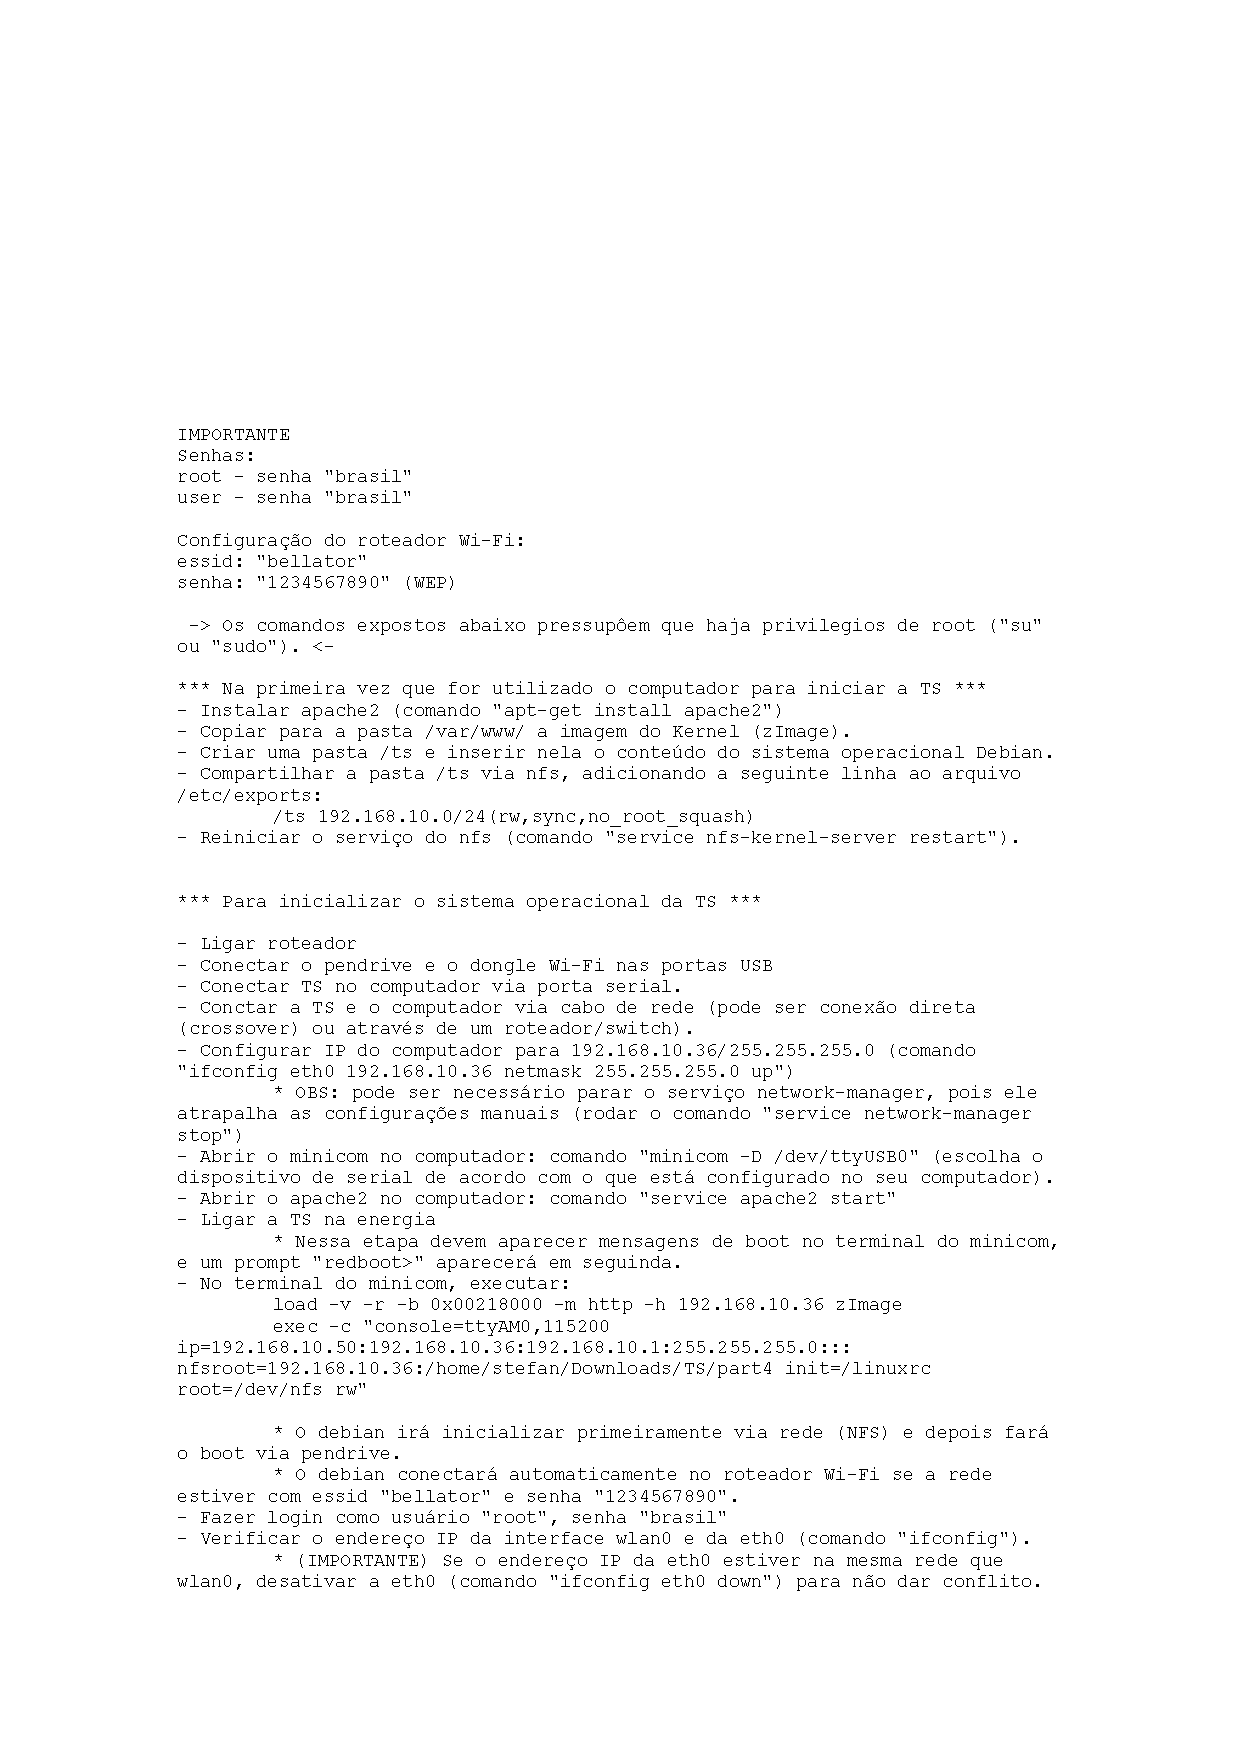
\includepdf[pagecommand=\chapter{Iniciando a ts}]{ini_ts.pdf}
\includepdf[pages=2, pagecommand=]{ini_ts.pdf}

\chapter{Conhecendo a estação-base}
É possível salvar os obstáculos identificados pelo robô bellator durante uma seção de testes em um arquivo \textit{.bellator}. Também é possível carregar os dados salvos no arquivo \textit{.bellator} no caso da retomada de uma seção de testes.

A seguir, é apresentada a interface gráfica da estação-base.

\begin{figure}[H]
\centering
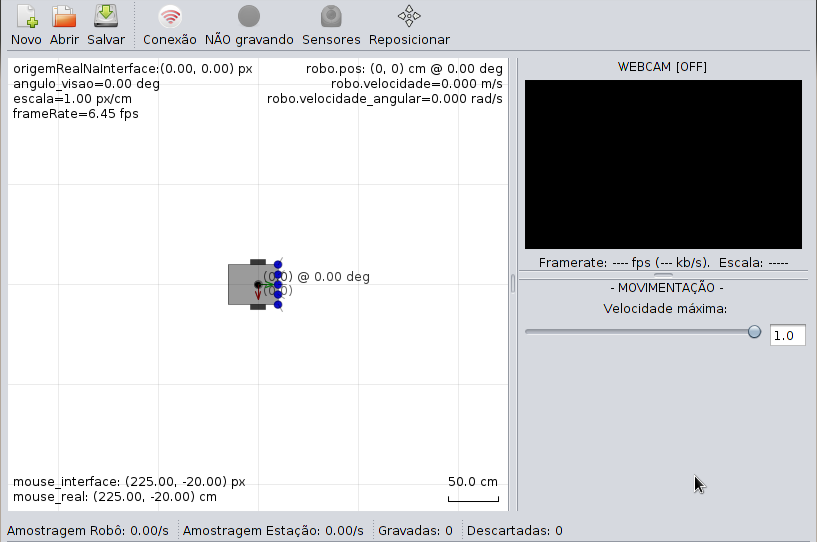
\includegraphics[width=\textwidth]{./images/interface_grafica.png}
\caption{Interface gráfica da estação-base}
\label{fig:ui}
\end{figure}

\begin{table}[H]
  \caption{Botões da interface gráfica e suas funcionalidades}
  \centering
  \begin{tabular}{p{2cm}p{12cm}}
    \toprule
    
\includegraphics[width=0.03\textwidth]{./images/document-new.png} & Inicia um novo arquivo no formato \textit{.bellator} \\
    
\includegraphics[width=0.03\textwidth]{./images/document-open.png} & Abre um arquivo salvo no formato \textit{.bellator} \\
    
\includegraphics[width=0.03\textwidth]{./images/document-save_24.png} & Salva um arquivo no formato \textit{.bellator} \\
    
\includegraphics[width=0.03\textwidth]{./images/camera-web.png} & Abre a janela de controle dos sensores, na qual é possível ajustar parâmetros dos sensores e da webcam. \\
    
\includegraphics[width=0.03\textwidth]{./images/wifi2-blue.png} & Quando acionado, indica que a conexão WI-FI está funcional \\
    
\includegraphics[width=0.03\textwidth]{./images/wifi2-red.png} &  Indica que a conexão WI-FI não está funcional \\
    
\includegraphics[width=0.03\textwidth]{./images/gtk-media-record.png} & Inicia a gravação dos obstáculos. Esta função só está disponível após o estabelecimento de uma conexão funcional com o robô.\\
    \hline
  \end{tabular}
  \label{tab:alternativas_desenho}
\end{table}

\begin{table}[H]
  \caption{Possíveis comandos de movimentos a serem enviados para o robô}
  \centering
  \begin{tabular}{p{2cm}p{8cm}}
    \toprule
    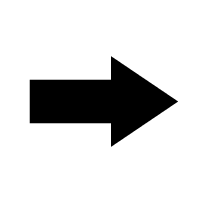
\includegraphics[width=0.05\textwidth]{./images/seta_direita.png} & Movimentar para direita \\
    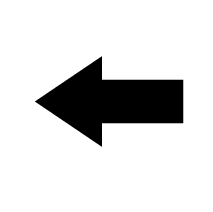
\includegraphics[width=0.05\textwidth]{./images/seta_esquerda.png} & Movimentar para a esquerda \\
    
\includegraphics[width=0.05\textwidth]{./images/seta_cima.png} & Movimentar para frente \\
    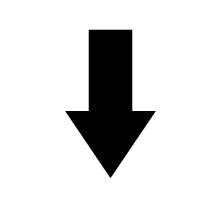
\includegraphics[width=0.05\textwidth]{./images/seta_baixo.png} & Movimentar para trás \\
    
\includegraphics[width=0.05\textwidth]{./images/curva_direita_cima.png} & Fazer curva para frente e à direita  \\
    
\includegraphics[width=0.05\textwidth]{./images/curva_direita_abaixo.png} & Fazer curva para trás e à direita \\
    
\includegraphics[width=0.05\textwidth]{./images/curva_esquerda_cima.png} & Fazer curva para frente e à esquerda \\
    
\includegraphics[width=0.05\textwidth]{./images/curva_esquerda_abaixo.png} & Fazer curva para trás e à esquerda  \\
    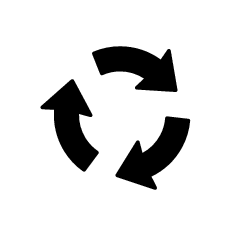
\includegraphics[width=0.05\textwidth]{./images/giro_horario.png} & Girar no sentido horário \\
    
\includegraphics[width=0.05\textwidth]{./images/giro_anti_horario.png} & Girar no sentido anti-horário \\
    \hline
  \end{tabular}
  \label{tab:alternativas_desenho}
\end{table}

\chapter{Conectando à estação-base}

Para que a estação base e o robô se conectem, a placa com o linux embarcado precisa estar ligada a pelo menos 30 segundos, para garantir que o sistema operacional da placa e o dongle WI-FI estejam plenamente funcionais. Tanto o computador, quanto o robô precisam estar na mesma rede WI-FI. Em seguida, é preciso acessar o software da estação-base e clicar em conectar. Na janela que aparecer, clicar em conectar novamente. A estação base exibirá uma mensagem informando que a conexão foi estabelecida com sucesso, conforme a Figura \ref{fig:conectado}.


\begin{figure}[H]
\centering
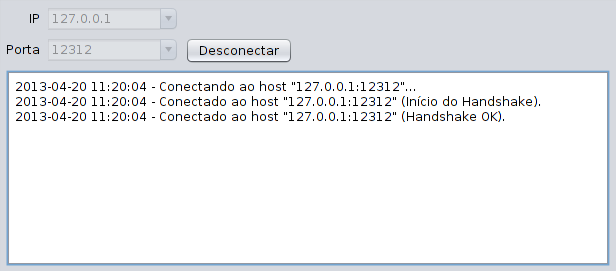
\includegraphics[width=\textwidth]{./images/conectado.png}
\caption{Mensagem de conexão com sucesso da estação-base}
\label{fig:conectado}
\end{figure}


\raggedright

\end{document}

